{% enclose the chapter in braces to limit the scope of defined commands
\newcommand{\exampleroot}{\noss{notebooks}}
\newcommand{\srcdir}{\noss{\exampleroot\bs src}}
\newcommand{\srgname}{\noss{srg}}
\newcommand{\srgfullname}{\noss{self_regulating_gene}}
\newcommand{\srgmfpt}{\noss{{\srgname}_mfpt}}
\newcommand{\dir}{\noss{\exampleroot\bs\srgmfpt}}

\newcommand{\data}{data}
\newcommand{\dataw}{\noss{{\data}_worked}}
\newcommand{\sbml}{{\srgfullname}.sbml}
\newcommand{\lm}{\srgname.lm}
\newcommand{\out}{\noss{{\srgname}_out.sfile}}
\newcommand{\lmlog}{\srgname.log}
\newcommand{\nb}{\srgmfpt.ipynb}
\newcommand{\nbw}{\noss{{\srgmfpt}_worked.ipynb}}
\newcommand{\plotter}{plotTiling.py}

\newcommand{\datapath}{\dir\bs\data}
\newcommand{\datawpath}{\dir\bs\dataw}
\newcommand{\sbmlpath}{\exampleroot\bs{\sbml}}
\newcommand{\lmpath}{\datapath\bs\lm}
\newcommand{\outpath}{\datapath\bs\out}
\newcommand{\lmlogpath}{\datapath\bs\lmlog}
\newcommand{\nbpath}{\exampleroot\bs\nb}
\newcommand{\nbwpath}{\exampleroot\bs\nbw}
\newcommand{\plotterpath}{\srcdir\bs\plotter}

\newcommand{\lmpathrel}{\data\bs\lm}
\newcommand{\outpathrel}{\data\bs\out}
\newcommand{\lmlogpathrel}{\data\bs\lmlog}

\chapter{Using FFPilot to calculate mean first passage time (MFPT): self regulating gene}

\section{Overview}

In this section I'll go over how to use FFPilot to calculate the \abr{MFPT} of the \abr{SRG}. \abr{SRG} consists of a single protein, which I'll call protein A. Protein A participates in a positive feedback loop in which it upregulates its own production. Additionally, it experiences constant degradation. These properties make \abr{SRG} bistable, and it will stochastically switch from one state, with low levels of protein A, to another, with high levels of protein, and back again over time.

\begin{center}
    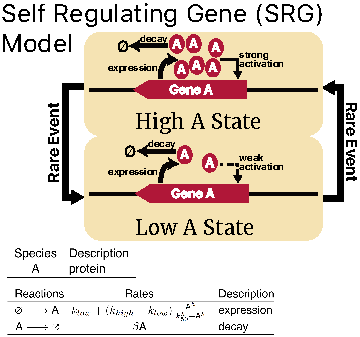
\includegraphics[width=5.0in]{{../Figures/model_schematics/self_regulating_gene}.pdf}
\end{center}

Starting from a \abr{SRG} model file included with this tutorial, \pth{\sbmlpath}, I'll show you how to set up the simulation input file, execute the simulation, and analyze the output. If you execute the example commands and code exactly as written, you should end up with a new directory \pth{\datapath} that contains \pth{\lm}, the simulation input file, and \pth{\out}, the simulation output file. Pre-made example input and output files can be found in \pth{\datawpath}.

\section{Input file setup}\label{sec:srg_mfpt_input_setup}
The input file for an FFPilot simulation is the same as for standard (\ie direct sampling) simulation. However, some extra information is required, in the form of an order parameter and a tiling. %Input can be prepared in a few steps:
%\begin{enumerate}
%    \item Convert \pth{\sbml} $\rightarrow$ \pth{\lm}.
%    \item\label{item:add_op} Add an order parameter. 
%    \item\label{item:add_tiling_srg} Add a tiling.
%    \item\label{item:add_es_opts} Add any simulation options. 
%\end{enumerate}

\subsection{Convert .sbml -> .lm}\label{sec:sbml_conversion_srg}
Models of biochemical systems are often distributed in the SBML format. These can be converted to the \pth{.lm} format required by Lattice Microbes using the \pth{lm_sbml_import} utility.

Open a terminal and \sh{cd} to the \pth{\dir} directory. You will then execute the following commands:

\inputcmd{snippets/srg_mfpt/lm_sbml_import.sh}

The first command creates a separate \pth{\datapath} directory which we will use to hold any simulation input/output that we produce during this section of the tutorial. The last command converts \pth{\sbmlpath} file using  \pth{lm_sbml_import} and then places the resulting \pth{.lm} file at \pth{\lmpath}.

\subsection{Add an order parameter}\label{sec:add_op}
If fed into \abr{LMES} in its current form, \pth{\lm} could be used to run a standard replicate simulation. However, in order to use \pth{\lm} as input for an FFPilot simulation, we'll have to first open it up and add some extra information: an order parameter and a tiling. We'll start with the order parameter.

Internally, \pth{.lm} files are based on the \keyword{hdf5} format. This means that all of the existing \keyword{hdf5} software tools can directly interact with \pth{\lm}, just the same as for any \keyword{hdf5} file. We'll be using two of these \keyword{hdf5} tools in this tutorial:
\begin{description}[style=nextline]
    \item[\py{h5py}] A Python package that can open and/or modify \keyword{hdf5} files from within Python code. We'll be using \py{h5py} to modify the input file/add the extra information.
    \item[\exe{h5dump}] A command line tool that can be used to dump the contents of a \keyword{hdf5} file in plain text to the \keyword{stdout} of a terminal. We'll be using \exe{h5dump} to show the correct format for the extra input required by FFPilot.
\end{description}

The order parameter that we will use with \abr{SRG}, which I will call $\oparama$, will just be the count of the single chemical species in the system, protein A. Order parameter $\oparama$ is a linear combination of species counts and can thus be represented in \abr{LMES} as a linear order parameter. The following Python script will open up \pth{\lm} and add the definition of $\oparama$ in the required format:

\inputpy{snippets/srg_mfpt/add_order_parameter.py}

The above script adds a new group, \code{OrderParameters}, to \pth{\lm}, the contents of which we can inspect using \exe{h5dump} by opening a terminal, \pth{cd}-ing to \pth{\dir}, and then running the following command:

\inputcmd{snippets/srg_mfpt/h5dump_order_parameter.sh}

The dump will show that the \code{OrderParameters} group contains one subgroup, \code{0}:

\begin{minted}{text}
HDF5 "data/srg.lm" {
GROUP "OrderParameters" {
   GROUP "0" {
\end{minted}

Group \code{OrderParameters\bs0} contains the definition of $\oparama$. Two attributes are set on group \code{0}, \code{\oparamid} and \code{\oparamtype}:
\begin{minted}{text}
      ATTRIBUTE "ID" {
         DATATYPE  H5T_STD_I64LE
         DATASPACE  SCALAR
         DATA {
         (0): 0
         }
      }
      ATTRIBUTE "Type" {
         DATATYPE  H5T_STD_I64LE
         DATASPACE  SCALAR
         DATA {
         (0): 0
         }
      }
\end{minted}
These attributes, which are required in every order parameter definition, do the following:
\begin{description}[style=nextline]
    \item[\code{\oparamid}] This attribute (which should match the name of the \code{OrderParameters} subgroup on which it is set) is the name by which \abr{LMES} will refer to $\oparama$ internally.
    \item[\code{\oparamtype}] This attribute tells \abr{LMES} what kind of order parameter this is, and how it should interpret the order parameter's definition when calculating its value. A \code{\oparamtype} of \code{0} tells \abr{LMES} that $\oparama$ is a linear order parameter.
\end{description}

Inside of group \code{0} are two 1D arrays (by convention, \keyword{hdf5} tools refer to arrays as datasets), \code{\oparamspecids} and \code{\oparamcoeffs}:
\begin{minted}{text}
      DATASET "SpeciesCoefficients" {
         DATATYPE  H5T_IEEE_F64LE
         DATASPACE  SIMPLE { ( 1 ) / ( 1 ) }
         DATA {
         (0): 1
         }
      }
      DATASET "SpeciesIDs" {
         DATATYPE  H5T_STD_I64LE
         DATASPACE  SIMPLE { ( 1 ) / ( 1 ) }
         DATA {
         (0): 0
         }
      }
\end{minted}
\abr{LMES} uses the values in these arrays to define the formula for the value of an order parameter. For any linear order parameter $\oparam$, \abr{LMES} will use the following formula to calculate its value:
\begin{equation}
\label{eq:oparam_linear}
    \oparam = \sum_{\ix=0}^{\mcode{len(\oparamspecids)} - 1} \mcode{\counts[\oparamspecids[i]]} * \mcode{\oparamcoeffs[i]}
\end{equation}
where \code{\counts} is a 1D array containing the present count of each species in the system being simulated. \eqref{eq:oparam_linear} can be simplified considerably for $\oparama$:
\begin{align}
    \oparama &= \mcode{\counts[\oparamspecids[0]]} * \mcode{\oparamcoeffs[0]} \nonumber \\
    \oparama &= \mcode{\counts[0]} \nonumber
\end{align}

\subsection{Add a tiling}\label{sec:add_tiling_srg}
Now we add a tiling to the self regulating gene. The tiling will be defined in terms of order parameter $\oparama$. In the previous section we added $\oparama$ to \pth{\lm} and gave it an \code{ID} of \code{0}. The following Python script will open up \pth{\lm} and add a new tiling with an \code{ID} of \code{0}:

\inputpy{snippets/srg_mfpt/add_tiling.py}

Once the script has run, we can inspect the contents of the newly added \code{Tilings} group in \pth{\lm} by opening a terminal, \sh{cd}-ing to \pth{\dir}, and then running the following command:

\inputcmd{snippets/srg_mfpt/h5dump_tiling.sh}

The dump shows one subgroup, \code{0}, in the \code{Tilings} group:
\begin{minted}{text}
HDF5 "data/srg.lm" {
GROUP "Tilings" {
   GROUP "0" {
\end{minted}

Group \code{Tilings\bs0} has three required attributes set on it:
\begin{minted}{text}
      ATTRIBUTE "ID" {
         DATATYPE  H5T_STD_I64LE
         DATASPACE  SCALAR
         DATA {
         (0): 0
         }
      }
      ATTRIBUTE "OrderParameterID" {
         DATATYPE  H5T_STD_I64LE
         DATASPACE  SCALAR
         DATA {
         (0): 0
         }
      }
      ATTRIBUTE "Type" {
         DATATYPE  H5T_STD_I64LE
         DATASPACE  SCALAR
         DATA {
         (0): 0
         }
      }
\end{minted}
the description of which are as follows:
\begin{description}[style=nextline]
    \item[\code{\tilingid}] This attribute (which should match the name of the \code{Tiling} subgroup on which it is set) is the name by which \abr{LMES} will refer to this tiling internally.
    \item[\code{\tilingtype}] A tiling \code{\tilingtype} of \code{0} tells \abr{LMES} that this is a 1D linear tiling\footnote{1D linear is the only kind of tiling currently implemented in \abr{LMES}. Thus, for now, this is just a placeholder value that should always be set to 0. In the future, more complex tilings, such as ones based on the Voronoi tessellation\cite{Dickson:2009gt}, may be implemented.}.
    \item[\code{\tilingopid}] The \code{\oparamid} of the order parameter (in this case, $\oparama$) that will be used in the definition of this tiling. Specifically, the placement of the edges that separate the tiles/bins of this tiling will be specified in terms of the tiling's order parameter.
\end{description}

Inside of group \code{Tilings/0} are a 2D array, \code{\tilingbasins}, and a 1D array, \code{\tilingedges}:
\begin{minted}{text}
      DATASET "Basins" {
         DATATYPE  H5T_STD_I64LE
         DATASPACE  SIMPLE { ( 2, 1 ) / ( 2, 1 ) }
         DATA {
         (0,0): 10,
         (1,0): 160
         }
      }
      DATASET "Edges" {
         DATATYPE  H5T_IEEE_F64LE
         DATASPACE  SIMPLE { ( 13 ) / ( 13 ) }
         DATA {
         (0): 23, 33.5833, 44.1667, 54.75, 65.3333, 75.9167, 86.5, 97.0833,
         (8): 107.667, 118.25, 128.833, 139.417, 150
         }
      }
\end{minted}
These arrays are used in the following way:
\begin{description}[style=nextline]
    \item[\code{\tilingedges}] Each entry in this array holds a single coordinate given in terms of the tiling's order parameter. \abr{LMES} builds up a tiling by placing edges at these coordinates. In turn, the tiles/bins themselves are defined as the space in between any two adjacent edges. The size of the \code{\tilingedges} array is directly related to the number of separate phases run during an FFPilot simulation. During each stage there will be exactly as many phases executed as there are edges in the tiling used to set up the stage.
    \item[\code{\tilingbasins}] An N x D array, where N is the count of basins and D is the total number of unique chemical species in your system. The basins (which are defined in terms of a model's complete state space) are the points in the state space of a system from which the initial trajectories of each stage (\ie the phase zero trajectories) will be launched. Each row in \code{\tilingbasins} is treated as a separate basin.
\end{description}

The rows in the \code{\tilingbasins} array determine where trajectories are started from during phase zero. One complete self-contained FFPilot simulation (\ie a pilot stage following by a production stage) will be executed for each basin specified in the simulation input's tiling. Thus, setting two different basins is a convenient way to run the simulations required to calculate the \abr{MFPT} of both the forward switch (low A $\rightarrow$ high A) and the reverse switch (high A $\rightarrow$ low A) of the \abr{SRG} model.

The Python script we used to create our tiling will have set up two basins. The initial basin is at 10 counts of protein A, corresponding to the low A state of \abr{SRG}. This is located in front of the zeroth edge of tiling (which sits at 23 counts of A). The other basin is at 160 counts of protein A, corresponding to the high A state of \abr{SRG}. This basin is located behind the last edge of the tiling (which sits at 150 counts of A). The following figure gives a sense of what the tiling actually looks like:

\begin{center}
    \includegraphics[width=6.0in]{{../Figures/srg_edges}.pdf}
\end{center}

\subsection{(advanced) FFPilot batch mode (multiple tilings)}

In normal usage, the input file for an FFPilot simulation should have exactly one tiling. However, FFPilot simulations can be run in large batches by specifying multiple tilings. In this case, each separate tiling will be treated as if it describes a separate simulation. In other words, an FFPilot simulation run using an input that contains M separate tilings is equivalent to running a batch of M separate FFPilot simulations.

NB: when creating an input file to use with FFPilot batch mode, each tiling should have its own unique \code{ID}.

\subsection{Customize FFPilot simulation options}\label{sec:customize_opts_srg}

FFPilot is designed to require as little user input as possible. All of the simulation options/parameters that FFPilot uses have reasonable (and, in some cases, adaptive) default values. On the other hand, FFPilot supports a number of options that can be used to control many different aspects of the simulation. In \pth{.lm} input files, options are set as attributes on the top level \code{Parameters} group. 

NB: \pth{lmes} only recognizes options set with values of type \code{str}. All non-string options (\ie \code{int}, \code{bool}, etc.) should be converted to \code{str} before they are set.

We'll set up some options for our FFPilot \abr{SRG} simulation using the following python script (which contains several examples of \code{str} conversion):

\inputpy{snippets/srg_mfpt/add_options.py}

In the above script, we set three options:
\begin{description}[style=nextline]
    \item[\code{ffluxPilotOutput}] \code{bool}, defaults to \code{False}. Turns on output of records from any pilot stages run during the simulation. Normally only simulation output from the production stages is saved, and the data from every pilot stage is discarded once its corresponding production stage has been set up. When this flag is set to \code{True}, however, output from both the pilot and the production stages is saved.
    \item[\code{errorGoal}] Percentage, specified as a \code{float} in the range \code{(0-1.0]}, defaults to \code{.05}. Sets a goal for the (percent) error in the overall basin-to-basin \abr{MFPT} calculated by each production stage. Based on the outcome of the preceding pilot stage, FFPilot automatically determines how many trajectories to launch in each phase of a production stage in order to achieve a sampling error at or below the set error goal. Set \code{errorGoal} to \code{.01} for a high accuracy simulation, or set it to \code{.10}+ for a relatively fast simulation.
\end{description}

\section{Running the simulation}\label{sec:running_srg_mfpt}
Now that the FFPilot input is prepared, you can execute the simulation by opening a terminal, \pth{cd}-ing to \pth{\dir}, and entering the following command:

\inputcmd{snippets/srg_mfpt/lmes.sh}

As shown above, running an FFPilot simulation requires two flags to be passed to the \abr{LMES} executable:
\begin{description}[style=nextline]
    \item[\code{-ffpilot}] Tells \abr{LMES} to run in FFPilot mode. Without this flag a default replicate simulation would be run instead.
    \item[\code{-f <input-path>}] Tells \abr{LMES} that the simulation input file can be found at \code{<input-path>}.
\end{description}

The path at which the simulation output will be saved is automatically determined from the input path. In this case, that means the simulation output will be saved to \pth{\outpathrel}. Alternatively, you can explicitly set the simulation output path by specifying the \code{-fo <output-path>} flag on the command line when you execute \abr{LMES}.

Since this simulation is set up using a relatively loose 10\% error goal, it should run to completion fairly quickly. When run on my laptop (3.1 GHz, 4 CPU cores), the simulation finishes in about 30 seconds.

\subsection{(advanced) Preserving the simulation log}
Normally, the \pth{lmes} simulation log gets dumped directly to the terminal as the simulation runs. You can instead preserve the log for later perusal by running \pth{lmes} with a slightly modified command:

\inputcmd{snippets/srg_mfpt/lmes_log.sh}

where we've saved the simulation log to \pth{\lmlogpath} using \sh{>}, the Linux redirection operator.

One downside of redirecting the log is that it will prevent any progress messages from getting printed out to the terminal, making it hard to tell if the simulation is running correctly. One workaround is to monitor the log file in real time using the \code{watch} command while the simulation adds to it:

\inputcmd{snippets/srg_mfpt/watch_log.sh}

where the \code{-n} flag controls the number of lines that are displayed.

\section{Analyzing the log}

As an \pth{lmes} simulation runs, an informative log is dumped to \pth{stdout}. Aside from helping to monitor simulation progress, a large quantity of information about the outcome of an FFPilot simulation can be gleaned from the simulation log alone. For example, the \abr{MFPT} estimate is printed out at the end of every stage, eliminating the need to dig around in the actual simulation output file for this value. As well, the log contains some unique metadata about the simulation, such as the total elapsed wall-clock time.
% \footnote{Do not be concerned if the lines of the log get printed on top of each other, or if a particular log message is printed out more than once. These behaviors are by design, and are not indicative of bugs in the simulation.}

\subsection{FFPilot simulation progress log messages}

FFPilot simulations, like all \pth{lmes} simulations, begin with a kickoff phase, during which input is parsed and all of the parallel processes are initialized and coordinated. Once the kickoff is complete (usually only a few seconds when running \pth{lmes} on a single computer), an FFPilot simulation begins in earnest with the start of the pilot stage, as signaled by the following line getting printed to the log:
\begin{minted}{text}
Forward Flux stage 0 started (tiling_id: 0, basin_id: 0, stage_type: Pilot)
\end{minted}
This type of progress message is printed out at the start of every simulation stage. Each comma-separated term in between the parentheses holds a piece of information about the current simulation stage:
\begin{description}[style=nextline]
    \item[\code{tiling_id}] This gives the \code{ID} of the tiling used to set up the simulation stage. This matches the \code{ID} of the tiling we created earlier (see \secref{sec:add_tiling_srg}), and confirms that it was used to set up this simulation stage.
    \item[\code{basin_id}] This corresponds to the row index of \code{\tilingbasins} from which the basin species counts for this stage were taken. These basin species counts will be used to initialize phase 0 trajectories during this stage.
    \item[\code{stage_type}] Tells you whether this is a pilot or a production stage. One of each kind of stage is run for each basin in each tiling present in the simulation input.
\end{description}

Another kind of progress message is printed out at the start of each phase zero:
\begin{minted}{text}
Forward Flux phase 0 started (zeroth_edge: 23.00, \
    phase_limit: FORWARD_FLUXES >= 10000.00)
\end{minted}
The terms in the parentheses give some information about how this phase will be executed:
\begin{description}[style=nextline]
    \item[\code{zeroth_edge}] The coordinate of the tiling edge (given in terms of the tiling's order parameter) closest to the basin in which this phase's trajectories are initialized. Each time a phase zero trajectory crosses the \code{zeroth_edge} while traveling away from its starting basin, the simulation counts this as a single forward flux event. Additionally, the state that the trajectory was in when it fluxed forward is added to the dictionary of starting states that will be used to initialize trajectories during phase 1.
    \item[\code{phase_limit}] Describes the condition that must be fulfilled in order for this phase to be considered complete. This particular \code{phase_limit} means that 10,000 forward flux events (summed across all phase zero trajectories) need to be observed before this phase will be terminated. Phase zero is always run using a \code{FORWARD_FLUXES} type \code{phase_limit}.
\end{description}

A slightly different progress message is printed out at the start of each phase $i>0$:
\begin{minted}{text}
Forward Flux phase 4 started (starting_edge: 54.75, goal_edge: 65.33, \
    phase_limit: FORWARD_FLUXES >= 10000.00)
\end{minted}
where the values in the parentheses mean:
\begin{description}[style=nextline]
    \item[\code{starting_edge}] The edge along which lies all of the starting states used to initialize trajectories during this stage.
    \item[\code{goal_edge}] Once a trajectory has been launched from \code{starting_edge} it will continue to run until it either crosses the \code{zeroth_edge} (as specified in the most recent phase zero progress message) or this \code{goal_edge}. In either case the simulation is immediately terminated. However, if the trajectory was stopped because it crossed the \code{goal_edge}, the simulation counts this as a forward flux event. As well, the state the trajectory was in when it fluxed forward is added to the dictionary of starting states that will be used to initialize trajectories in the next phase.
\end{description}
The \code{phase_limit} term means the same thing in the phases $i>0$ progress messages as it does in the phase zero progress message. However, unlike phase zero, the type of \code{phase_limit} used to run any given phase $i>0$ varies depending on whether the phase is part of a pilot or a production stage. Essentially, the type of the \code{phase_limit} determines the phase's termination condition:
\begin{description}[style=nextline]
    \item[\code{FORWARD_FLUXES >= n}] 
    The type of \code{phase_limit} used during pilot stages. Each phase $i>0$ will only be considered complete once \code{n} forward flux events (\ie the count of trajectories that reached the \code{goal_edge}) have been observed, regardless of how many trajectories have been launched in total.
    \item[\code{TRAJECTORY_COUNT >= n}] 
    The type of \code{phase_limit} used during production stages. Each phase $i>0$ is considered complete once the total number of trajectories that have been launched and run to termination is \code{n}.
\end{description}

\subsection{Stage outcome log messages}

Every time a pilot stage finishes, some of the highlights from its output are added to the log file:
\begin{minted}{text}
The phase costs are:
[4.62, 0.151, 1.61, 2.41, 2.72, 2.09, 1.65, 1.22, 0.967, 1.01, 0.951, 1.25, 1.5]
The phase weight sample variances are:
[152, 0.018, 0.12, 0.228, 0.245, 0.155, 0.0665, 0.0211, 0.00473, 0.00296, \
    0.000693, 0.000495, 0.000396]
Conservative estimates of the phase weights are:
[4.62, 0.0179, 0.137, 0.345, 0.56, 0.8, 0.922, 0.974, 0.993, 0.995, 0.998, \
    0.998, 0.999]
Attempting to achieve error goal 0.05 (confidence level 0.95) \
    with the following optimized trajectory counts:
[32385, 497266, 51746, 23142, 14016, 9022, 5917, 3830, 2210, 1792, 1148, 1000, 1000]
\end{minted}
\begin{description}[style=nextline]
    \item[phase costs] The $i$th entry of this array holds the average cost, in terms of the internal simulation time, of collecting a single sample (\ie observation of a forward flux event) during phase $i$.  
    \item[variances] The $i$th entry of this array holds the variance of the samples collected during phase $i$. The samples in question are used to estimate the phase weights at the end of each phase.
    \item[conservative weight estimates] The $i$th entry of this array holds the estimate of phase weight $i$ that is calculated at the end of each phase $i$.  of the samples collected during phase $i$.
\end{description}

The values in these first 3 arrays are used to parameterize the FFPilot optimizing equation\todo{add ref to my paper in submission}. The FFPilot optimizing is used to predict the optimal simulation plan (\ie count of trajectories to launch in each phase) for the upcoming production stage. By optimal, I mean the simulation plan that will achieve the specified error goal with the least computational effort possible. 

The reason why the weight estimates shown above are referred to as "conservative" is that, following their initial calculation, they have each been run through a set of biased estimators. These biased estimators have been designed such that when the conservative weight estimates are used to parameterize the FFPilot optimizing equation, the optimizing equation is in turn slightly biased towards overestimating the number of trajectories required to achieve the error goal. This has the beneficial effect of helping to ensure overall simulation accuracy, albeit at a small cost in computational efficiency. 

The last array in the pilot stage output log message contains the prediction of the FFPilot optimizing equation, given the values in the first 3 arrays:
\begin{description}[style=nextline]
    \item[optimized trajectory counts]
    The trajectory counts in this array are used to set up the \code{phase_limits} during the pilot stage. In other words, each phase $i>0$ of the production stage will be run until the count of trajectories that have run to completion reaches \code{optimized_trajectory_counts[i]}.
\end{description}

Each production stage also adds some the highlights from its results to the log once it finishes:
\begin{minted}{text}
The phase costs are:
[4.72, 0.151, 1.58, 2.42, 2.71, 2.08, 1.66, 1.28, 1.02, 1.03, 0.974, 1.24, 1.49]
The phase weights are:
[4.72, 0.0186, 0.145, 0.353, 0.573, 0.814, 0.926, 0.977, 0.993, 0.998, 1, 1, 1]
The first passage times to each tile edge are:
[4.72, 254, 1.76e+03, 4.97e+03, 8.67e+03, 1.07e+04, 1.15e+04, 1.18e+04, 1.19e+04, \
    1.19e+04, 1.19e+04, 1.19e+04, 1.19e+04]
The overall first passage time from the starting basin to the last tile edge is:
1.19e+04
\end{minted}

\begin{description}[style=nextline]
    \item[phase costs and weights]
    Same as from the pilot stage, but produced by the more accurate production stage.
    \item[mean first passage times] The $i$th entry in this array is the expected value of the time it takes to get from the simulation's starting basin to the $i$th edge of the tiling.
    \item[overall mean first passage time] The expected value of the time it takes to get from the simulation's starting basin to the ending basin. Equivalent to the final entry in the \abr{MFPT} array printed above. The basins can be thought of as the metastable states of the system, so the overall \abr{MFPT} can also be thought of as the inverse of the switching rate between those states.
\end{description}

\section{Browsing FFPilot output with dumpSFile}

Output from an FFPilot simulation takes the form of an \keyword{SFile}. By default, given that your simulation input is named \pth{<fname>.lm} the output is saved to \pth{<fname>_-_out.sfile} (this can be overridden by setting the \code{-fo <output-name>} cmd line option when running \abr{LMES}). \keyword{SFile} is a binary file format that holds information in the form of records. Each record begins with a short metadata section (record name, record type, data size in bytes) followed by a data section. For \abr{LMES} output in the \keyword{SFile} format, the data section takes the form of a serialized \href{https://developers.google.com/protocol-buffers/}{protocol buffer} message.

Although \keyword{SFiles} are not human readable, the \exe{dumpSFile} tool provided by the \code{robertslab} Python package can be used to easily view the contents of any \keyword{SFile}. For each record in an \keyword{SFile}, \exe{dumpSFile} converts the metadata into a human readable format, deserializes and formats the data portion, and then prints the results to \code{stdout}. The following command will dump the entire contents of \pth{\outpathrel} to the terminal:

\inputcmd{snippets/srg_mfpt/dump_all.sh}

The output will look something like this:

\inputout[fontsize=\tiny]{snippets/srg_mfpt/dump_all.txt}

The reason why the short simulation we just ran produced so much data is that we had turned on extra output via the \code{ffluxPilotOutput} option\footnote{If the simulation had been run using the default output options, the output would contain only 2 records, the summaries from each of the production stages.}. 

For each record it finds, \exe{dumpSFile} will first print out a line containing the record's metadata. This metadata has the following format:
\begin{minted}{text}
record.name    record.dataType    record.dataSize
\end{minted}
The data section of the record will then be printed out starting on the next line after the metadata.

\exe{dumpSFile} has many options that can help to tame the torrent of data. Here's a couple of the more useful ones:
\begin{description}[style=nextline]
    \item[\code{-i/--include <pattern0> <pattern1> ...}]
        When this option is set, \exe{dumpSFile} will attempt to match each regular expression \code{<patterni>} to each record. Records will only be printed out if  every pattern matches either the record's \code{name} or its \code{dataType}. Otherwise, \exe{dumpSFile} will skip the record. Patterns passed to \code{-i} are case insensitive.
        
        For example, the following \exe{dumpSFile} command, which passes the terms "summary", \\"production", and "basins/1"  to the \code{-i} flag:
        
        \inputcmd[fontsize=\footnotesize]{snippets/srg_mfpt/dump_include.sh}
        
        The "basins/1" and "production" terms match to \code{record.name}, and the "summary" term matches to \code{record.dataType}. This limits output to a single stage summary record, the one from the production stage that was initialized in basin \code{ID} \code{0}:
        
        \inputout[fontsize=\tiny]{snippets/srg_mfpt/dump_include.txt}
    
    \item[\code{-e/--exclude <pattern0> <pattern1> ...}]
        The opposite of \code{-i/--include}. Records will be excluded if every \code{<patterni>} matches either its \code{name} or its \code{dataType}.
    
    \item[\code{-l/--list-only}]
        When this flag is passed to \exe{dumpSFile}, only the metadata line of each record is printed out. This can be very useful for getting a sense of the complete contents of an \keyword{SFile}. It can also be combined with the \code{--exclude/--include} options.
        
        For example, the following command:
        
        \inputcmd{snippets/srg_mfpt/dump_metadata.sh}
        
        will output only the metadata from the pilot stage records:
        
        \inputout[fontsize=\tiny]{snippets/srg_mfpt/dump_metadata.txt}
        
\end{description}

Run \sh{dumpSFile --help} to get a detailed description of all of the options that \exe{dumpSFile} supports.

\section{Analyzing FFPilot output data using the robertslab.sfile Python package}

\subsection{Fetching and analyzing MFPT values in FFPilot simulation output}\label{sec:fetch_mfpt_srg}

Although \exe{dumpSFile} offers an easy way to browse the contents of FFPilot simulation output, it is less than ideal when used as a tool to perform detailed analysis. When performing any non-trivial calculations on FFPilot simulation output, the current recommended best practice is to use the \code{robertslab.sfile} Python package.

In this section I will go over how to retrieve and analyze data from an FFPilot output file using Python code. Specifically, I will walk you through the steps required to fetch the phase weights and \abr{MFPT}s from the production stage summary records, and show you how to recalculate the \abr{MFPT}s from the phase weights. 

As can seen in the output of \exe{dumpSFile} in the previous section, stage summary records each contain 4 arrays: 
\begin{description}[style=nextline]
    \item[\code{edges}] The positions of the edges in the tiling used to run the stage that produced this output.
    \item[\code{costs}] The mean computational cost per-trajectory launched during each phase in this stage. 
    \item[\code{first_passage_times}] The expected value of the simulation time required to reach each tiling edge from the starting basin.
    \item[\code{weights}] The phase weights. 
\end{description}

For this exercise we want the stage summary records from the two production stages. These records can be fetched from \pth{\out} with the following Python script:
\inputpy{snippets/srg_mfpt/ingest_output.py}

A simple plot of the \abr{MFPT} data can be made using the \code{matplotlib} Python plotting package:
\inputpy{snippets/srg_mfpt/plot_simple.py}
\begin{center}
    \includegraphics[width=6.0in]{{../Figures/srg_edge_mfpt_simple}.pdf}
\end{center}

The plot can be made much nicer with a bit of configuration:

\begin{center}
    \includegraphics[width=6.0in]{{../Figures/srg_edge_mfpt}.pdf}
\end{center}

the details of which are outside of the scope of this tutorial. However, for the curious, the complete code used to produce the above figure can be found in \pth{\plotterpath}, and a concrete example of its use is in the \pth{\nbpath} notebook.

\subsection{Calculating the MFPT to each tiling edge from the phase weights}

FFPilot simulation calculates the \abr{MFPT} to the $i$th edge of the tiling via a combination of the phase weights, $$\frac{w_0}{\prod_{i=1}^{j} w_i}$$ (as per \eqref{eq:mfpt_from_weights}).
The value of this formula at all of the edges can be quickly calculated using a cumulative product. Given a sequence in which the zeroth term is $w_0$ and remaining terms are the inverse values each $w_{i>0}$, the $i$th element of the cumulative product of this sequence will be the expected value of the time required to reach the $i$th edge:
\begin{equation*}
    \text{cumprod}(\{ w_0, \frac{1}{w_1}, \frac{1}{w_2}, \cdots, \frac{1}{w_N} \}) = \{ w_0, \frac{w_0}{w_1}, \frac{w_0}{w_1 w_2}, \cdots, \frac{w_0}{\prod_{i=1}^N w_i} \}
\end{equation*}

The \code{sfile} package, in conjunction with \code{numpy}, can be used to easily apply this formula:

\inputpy{snippets/srg_mfpt/recalc_mfpt.py}

If you then plot the recalculated \abr{MFPT} values against the \abr{MFPT} values that were originally present in the output file you get:

\begin{center}
    \includegraphics[width=6.0in]{{../Figures/srg_edge_mfpt_recalc}.pdf}
\end{center}

demonstrating that they are indeed identical.

}